% !TeX spellcheck = en_US
% !TEX root = ../thesis-example.tex
%
\section{Light Environment Reproduction}

To conclude all rendering steps taken by now: We have successfully created an 
image composition with correct projection parameters, recalculated a planar 
depth, synchronized in-engine frames with the camera input lag and realigned 
the frame rate between both image generating systems and cut off all overshot 
pixels that were recorded outside of the green screen.

\begin{figure}[htb]
	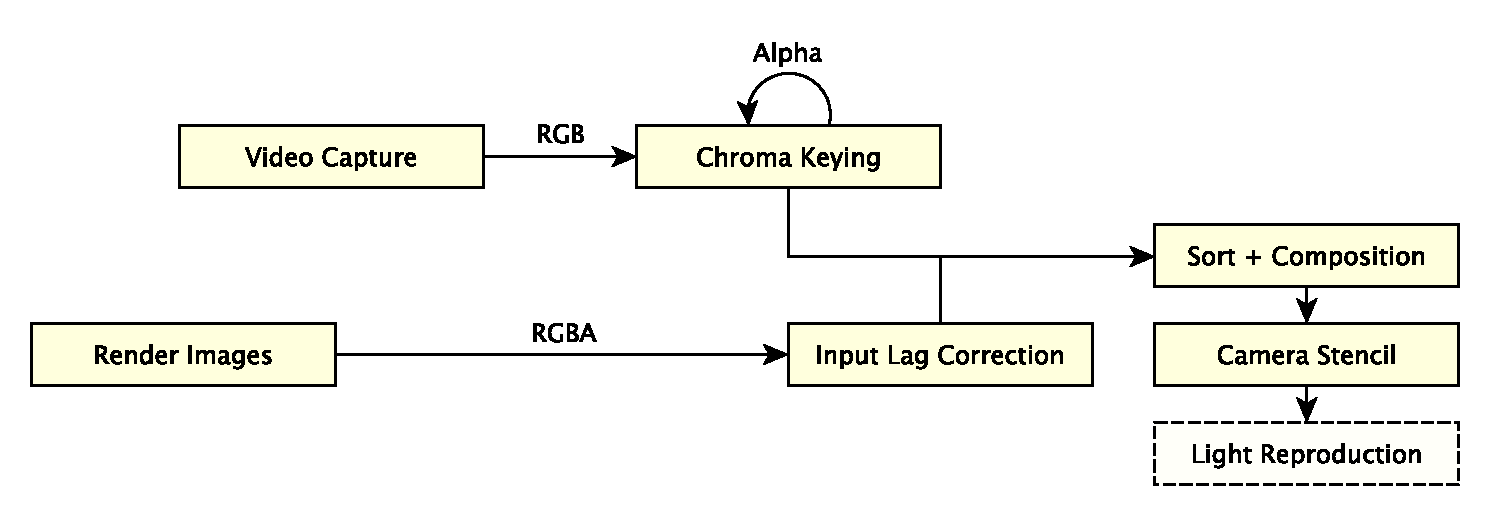
\includegraphics[width=\textwidth]{gfx/pipeline/4_7_lights.pdf}
	\caption{Following in this pipeline is lights reproduction}
	\label{fig:steps:lights}
\end{figure}

A minor last step is light-reproduction, in which an approximate lightning 
setting will be transferred from 3D environment to the video feed of a VR 
actor. Assuming that the video footage contains a natural lit, tint-free and 
calibrated video signal, it is possible to approximate how a VR actor would 
be lit like if he truly is inside the virtual environment (eg. fig. 
\ref{fig:light-reconstruction:actor}).

\begin{figure}[htbp]
	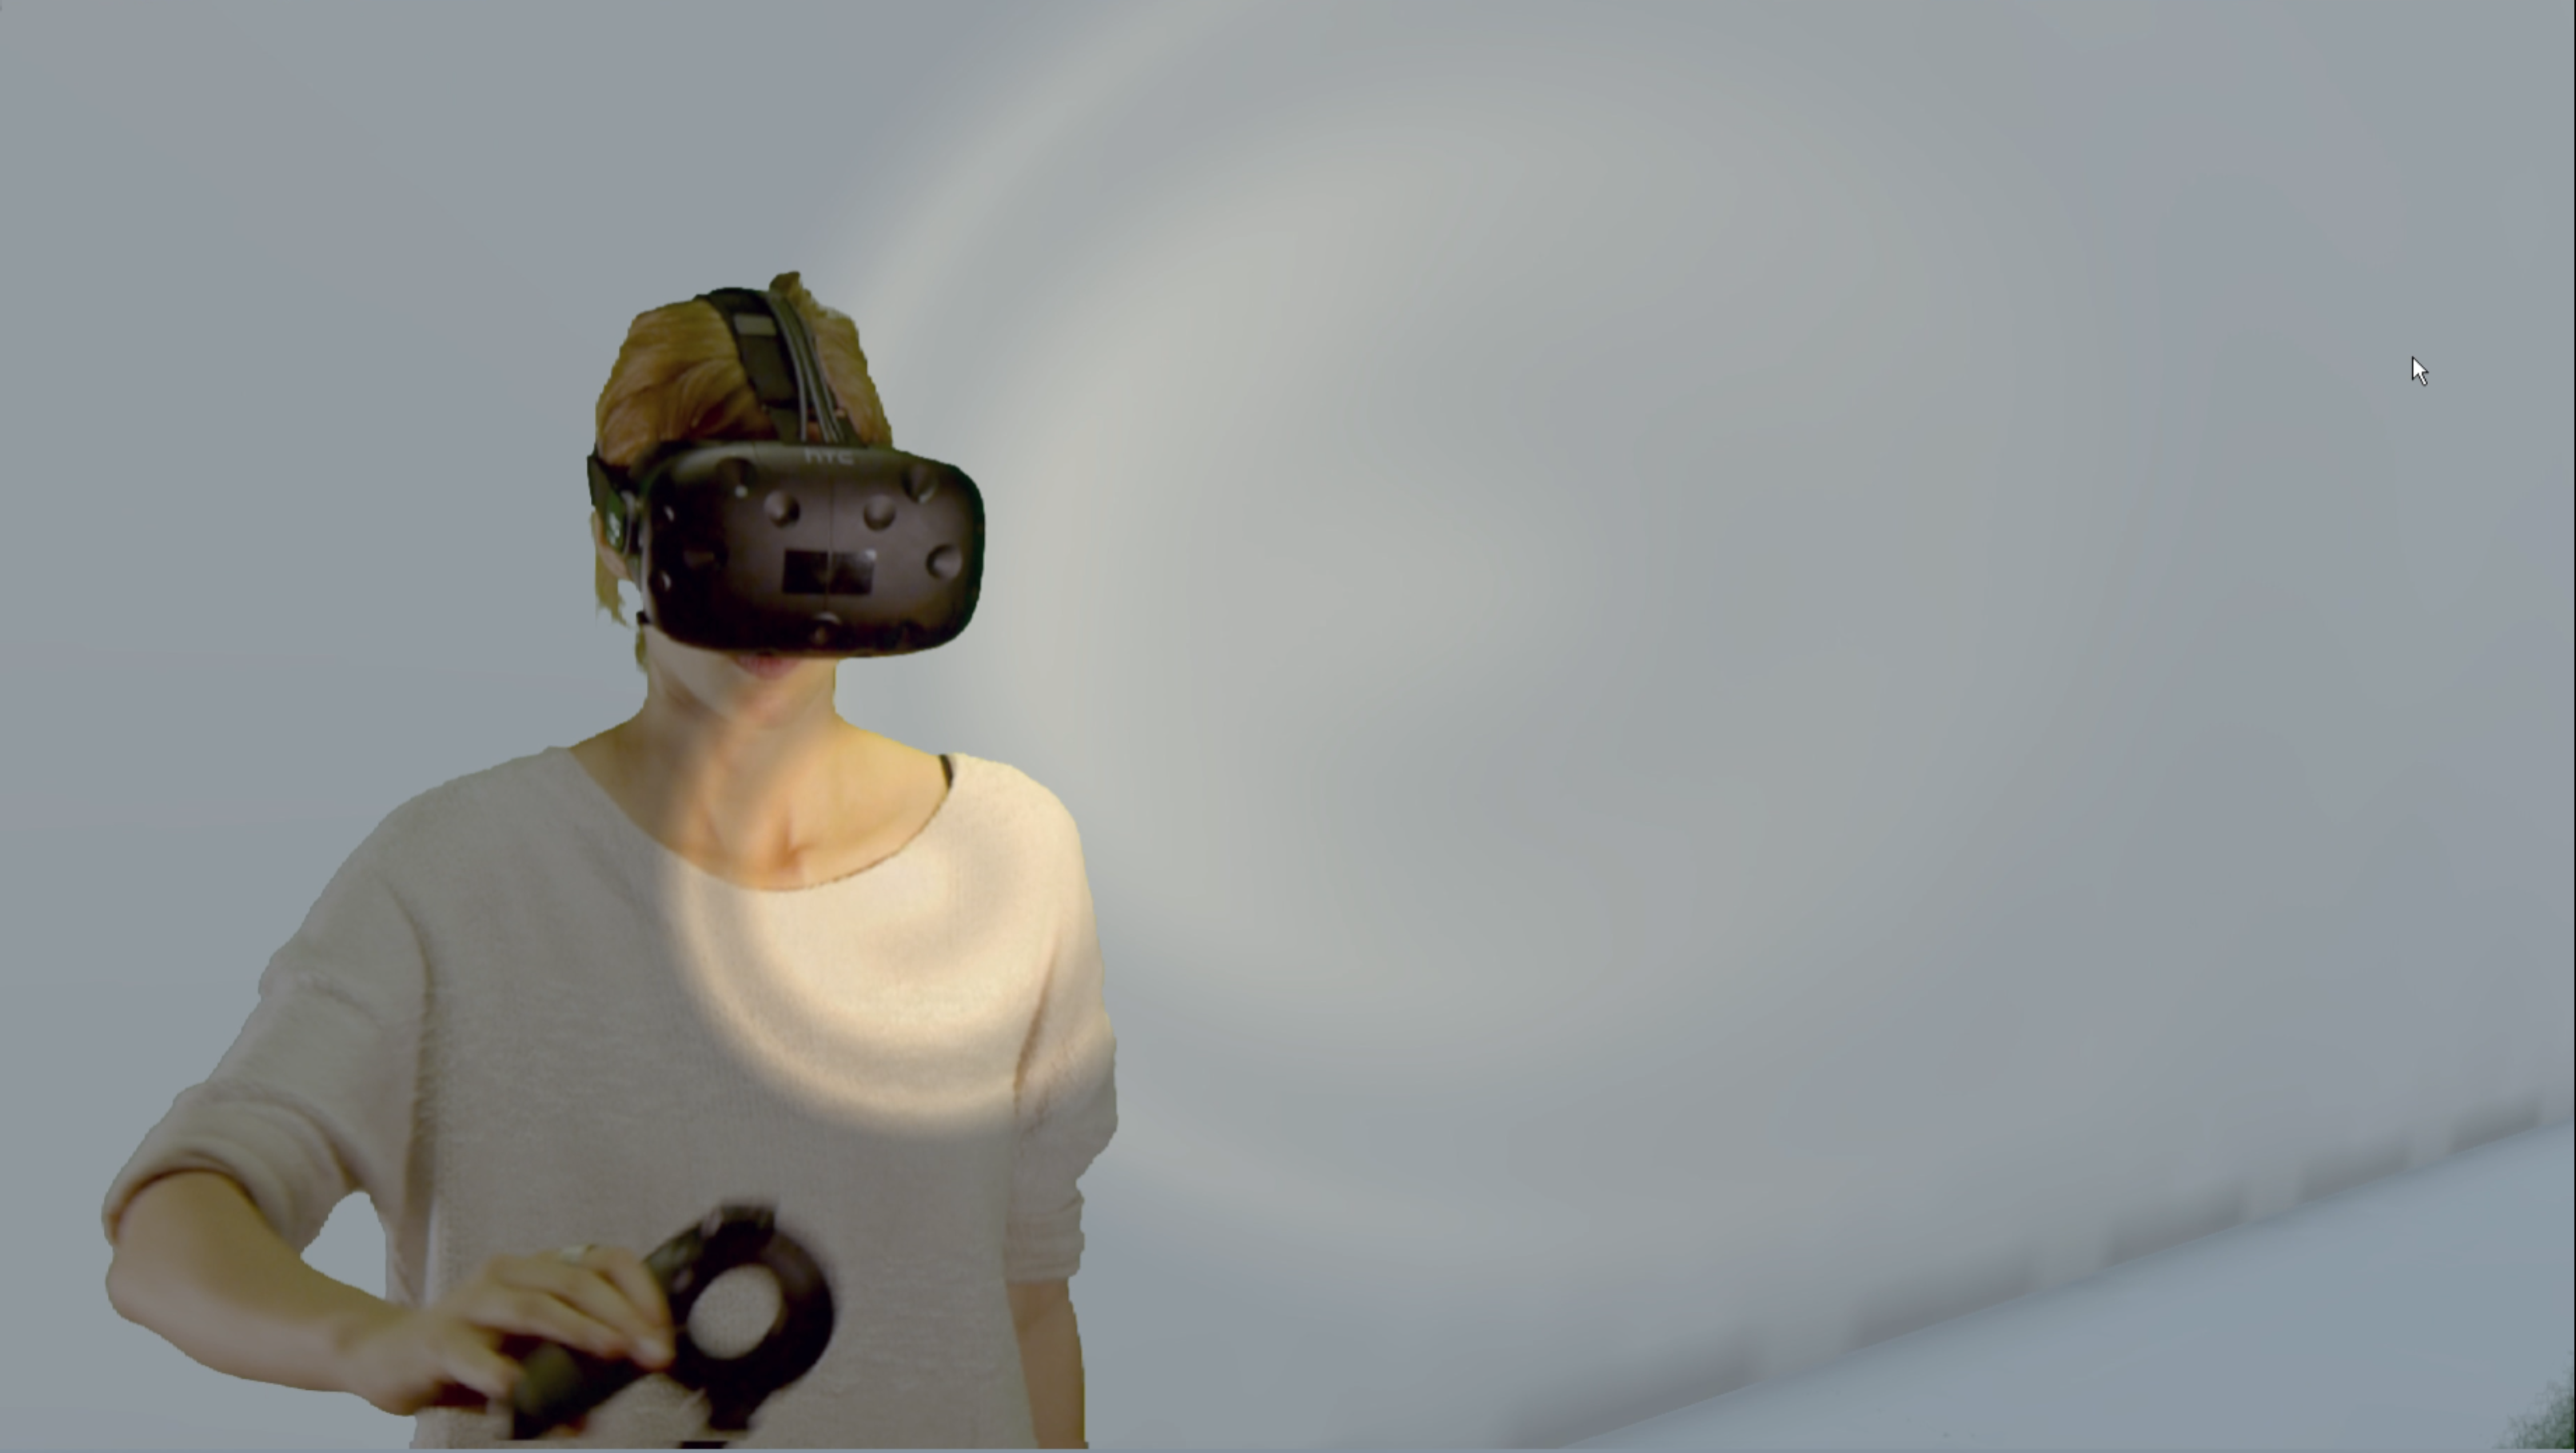
\includegraphics[width=\textwidth]{gfx/recoloring/self-illu.png}
	\caption{VR actress illuminates herself with a virtual flashlight}
	\label{fig:light-reconstruction:actor}
\end{figure}

Ambient light reproduction hinges on two assumptions: An actor's recorded video 
is flat for this purpose \textit{and} he receives clean and consistent light 
from all angles that has no additional glossiness. With that we can project a 
plane at the actor's position, filling the frustum edges of another virtual 
camera with the same camera projection parameters from section 
\ref{sec:projection-params}. This plane contains a simple lit material with 
white albedo coloring, which captures the lightning situation at this given 
point.

\begin{figure}[htb]
	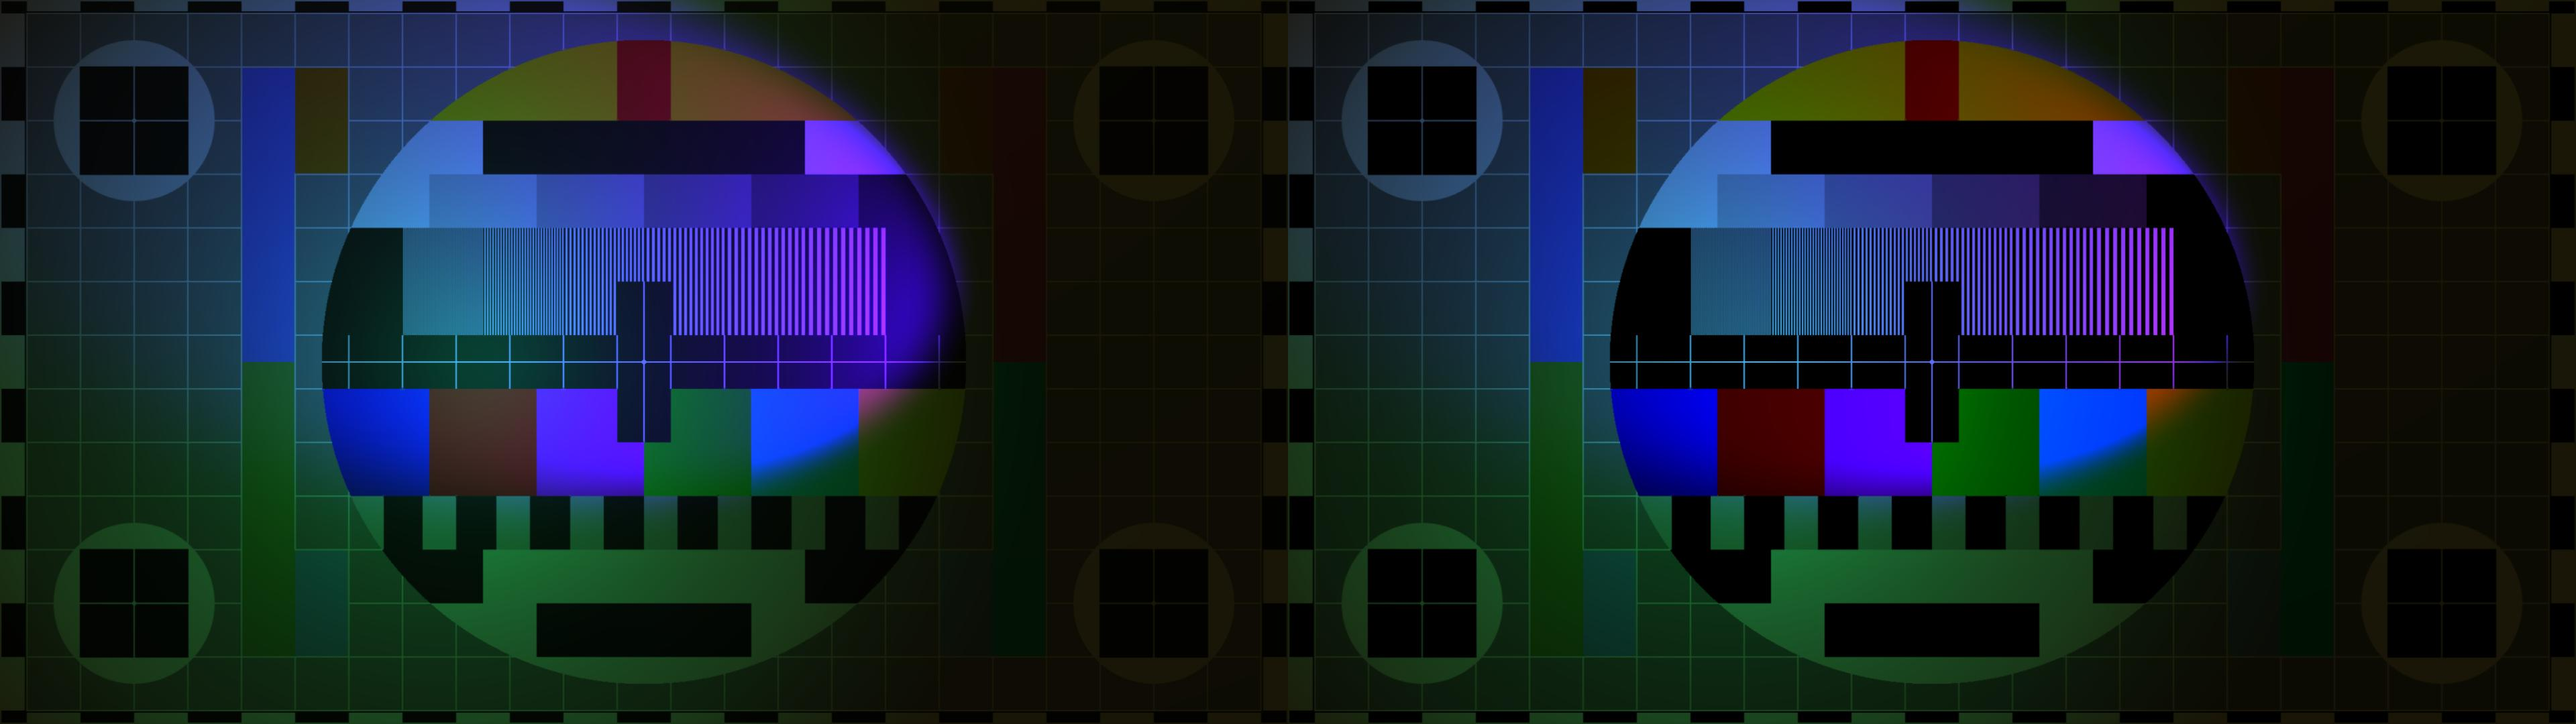
\includegraphics[width=\textwidth]{gfx/recoloring/comparison.jpg}
	\caption{Left: original, Right: reconstruction}
	\label{fig:light-reconstruction:diff-capture}
\end{figure}

To calculate the position $P_{pos}$ and size $\vec{P_{x, y}}$ with a 
given forward vector $\vec{C_{forward}}$ and position $C_{pos}$ of the 
camera, as well as a distance $Z$ between camera and actor and a current Field 
of View $FoV$ in radians by assuming a 16:9 video feed:

\eq{eq:light-reproduction:pos}{
	P_{pos} = C_{pos} + Z * \vec{C_{forward}}
}

\eq{eq:light-reproduction:size:1}{
	P_{x, y} =
	\begin{bmatrix}
		2 * \tan(FoV / 2) * Z \\
		P_{x} * \frac{16}{9}
	\end{bmatrix}	
}

These parameters can directly be applied to the transformation of said white 
plane which then captures the lightning environment inside the virtual scenes. 
As with all other composition-renderings, this step will be stored as a 
separate \code{RenderTexture} too and can operate on lower resolutions to speed 
up color and light sampling for performance gains.
\newline
The resulting frame buffer will be multiplied later onto the camera feed with a 
video color $C_V$ and the light plane $C_L$:

\eq{eq:light-reproduction:composition}{
	C_T = 
	\begin{bmatrix}
		C_{V_R} * C_{L_R} \\
		C_{V_G} * C_{L_G} \\
		C_{V_B} * C_{L_B}
	\end{bmatrix}
}

Lastly, a directional light with the same culling mask can be applied, to 
improve the overall brightness of this light mask to allow for more natural 
tint than a linear color operation.
